%
% p.tex -- slide template
%
% (c) 2021 Prof Dr Andreas Müller, OST Ostschweizer Fachhochschule
%
\bgroup
\begin{frame}[t]
\setlength{\abovedisplayskip}{5pt}
\setlength{\belowdisplayskip}{5pt}
\frametitle{Platonische Körper}
\vspace{-20pt}
\begin{columns}[t,onlytextwidth]
\begin{column}{0.33\textwidth}
\begin{block}{$T = T_h \cap \operatorname{SO(3)}$}
\begin{center}
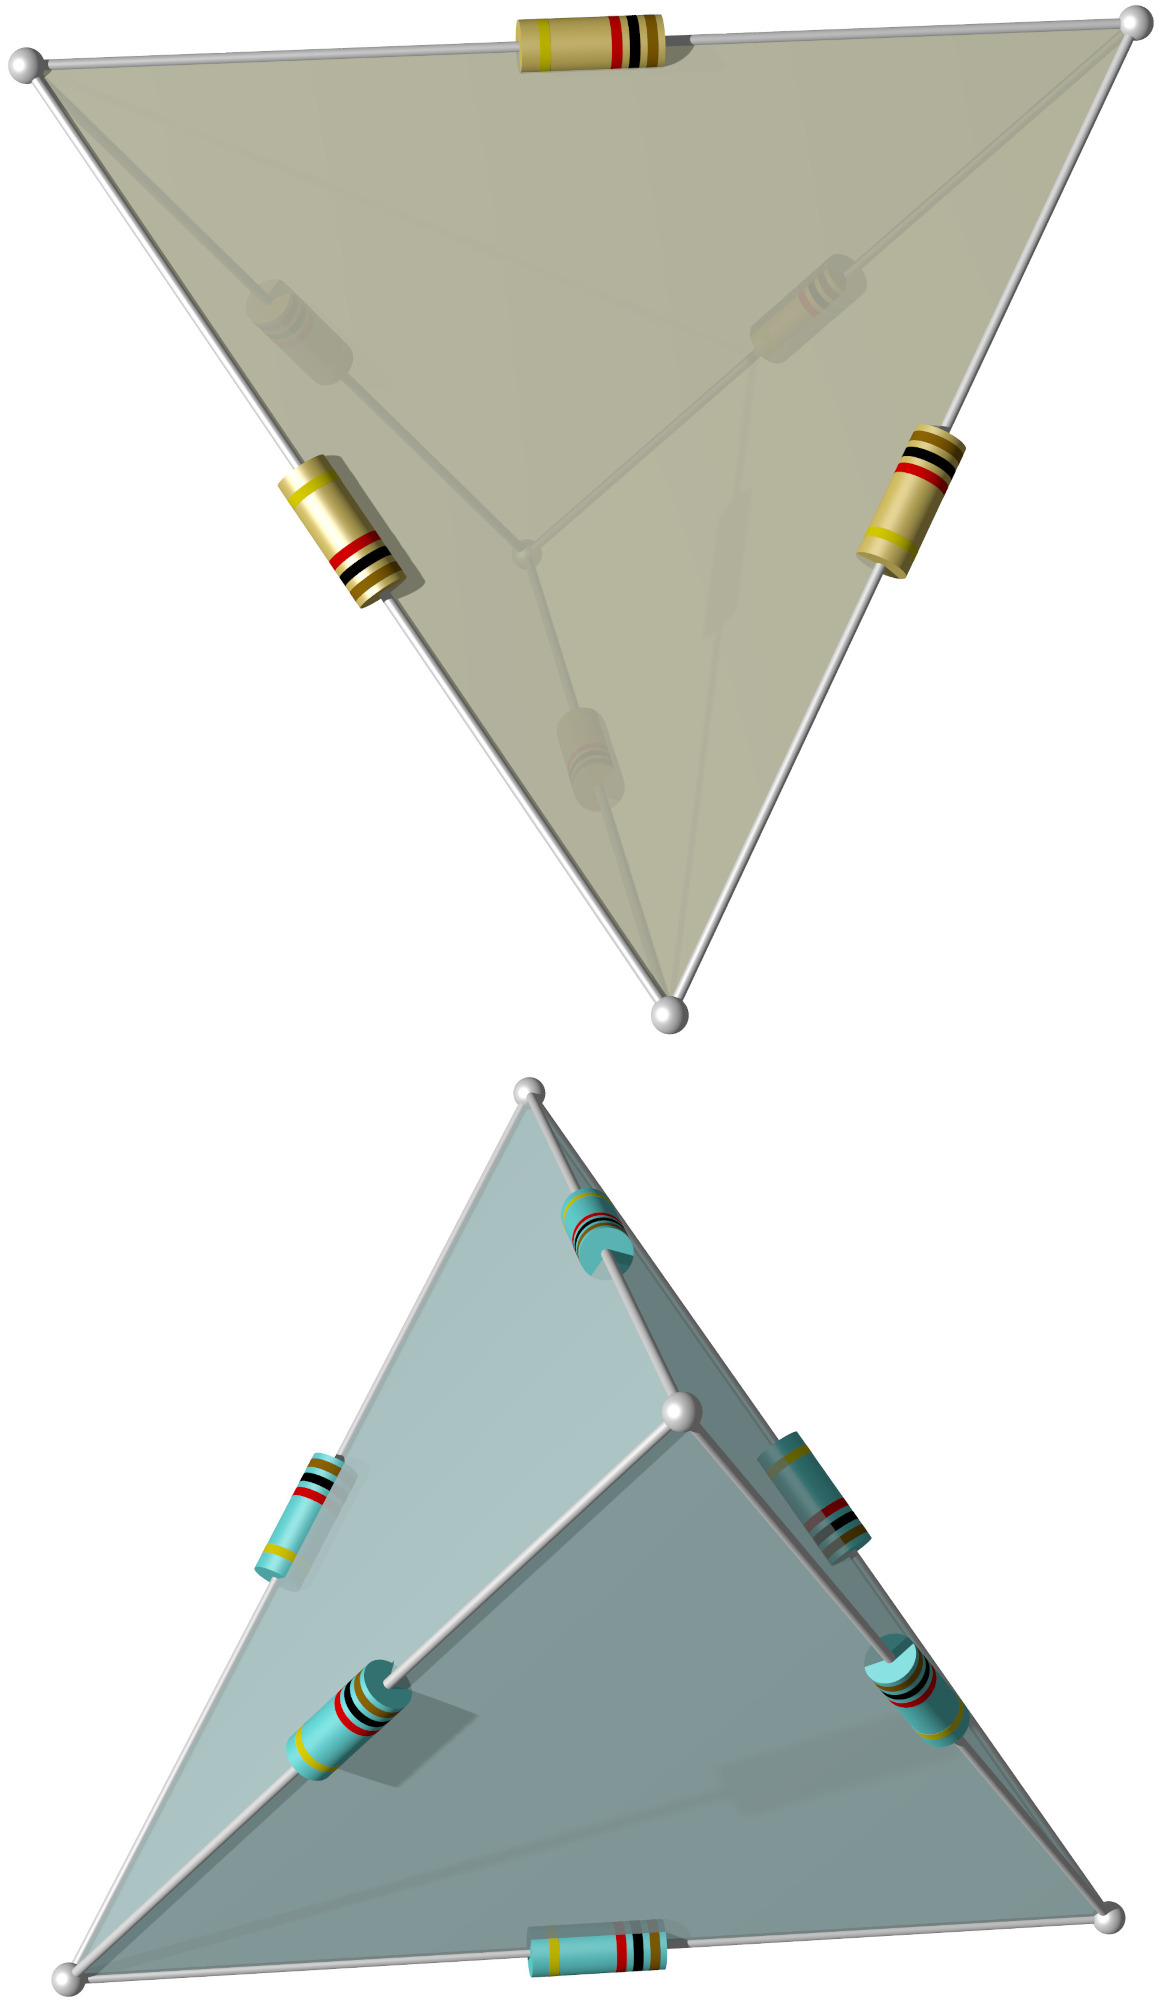
\includegraphics[width=0.8\textwidth]{../slides/6/punktgruppen/toi/T.jpg}
\end{center}
\end{block}
\end{column}
\begin{column}{0.33\textwidth}
\uncover<2->{%
\begin{block}{$O = O_h \cap \operatorname{SO(3)}$}
\begin{center}
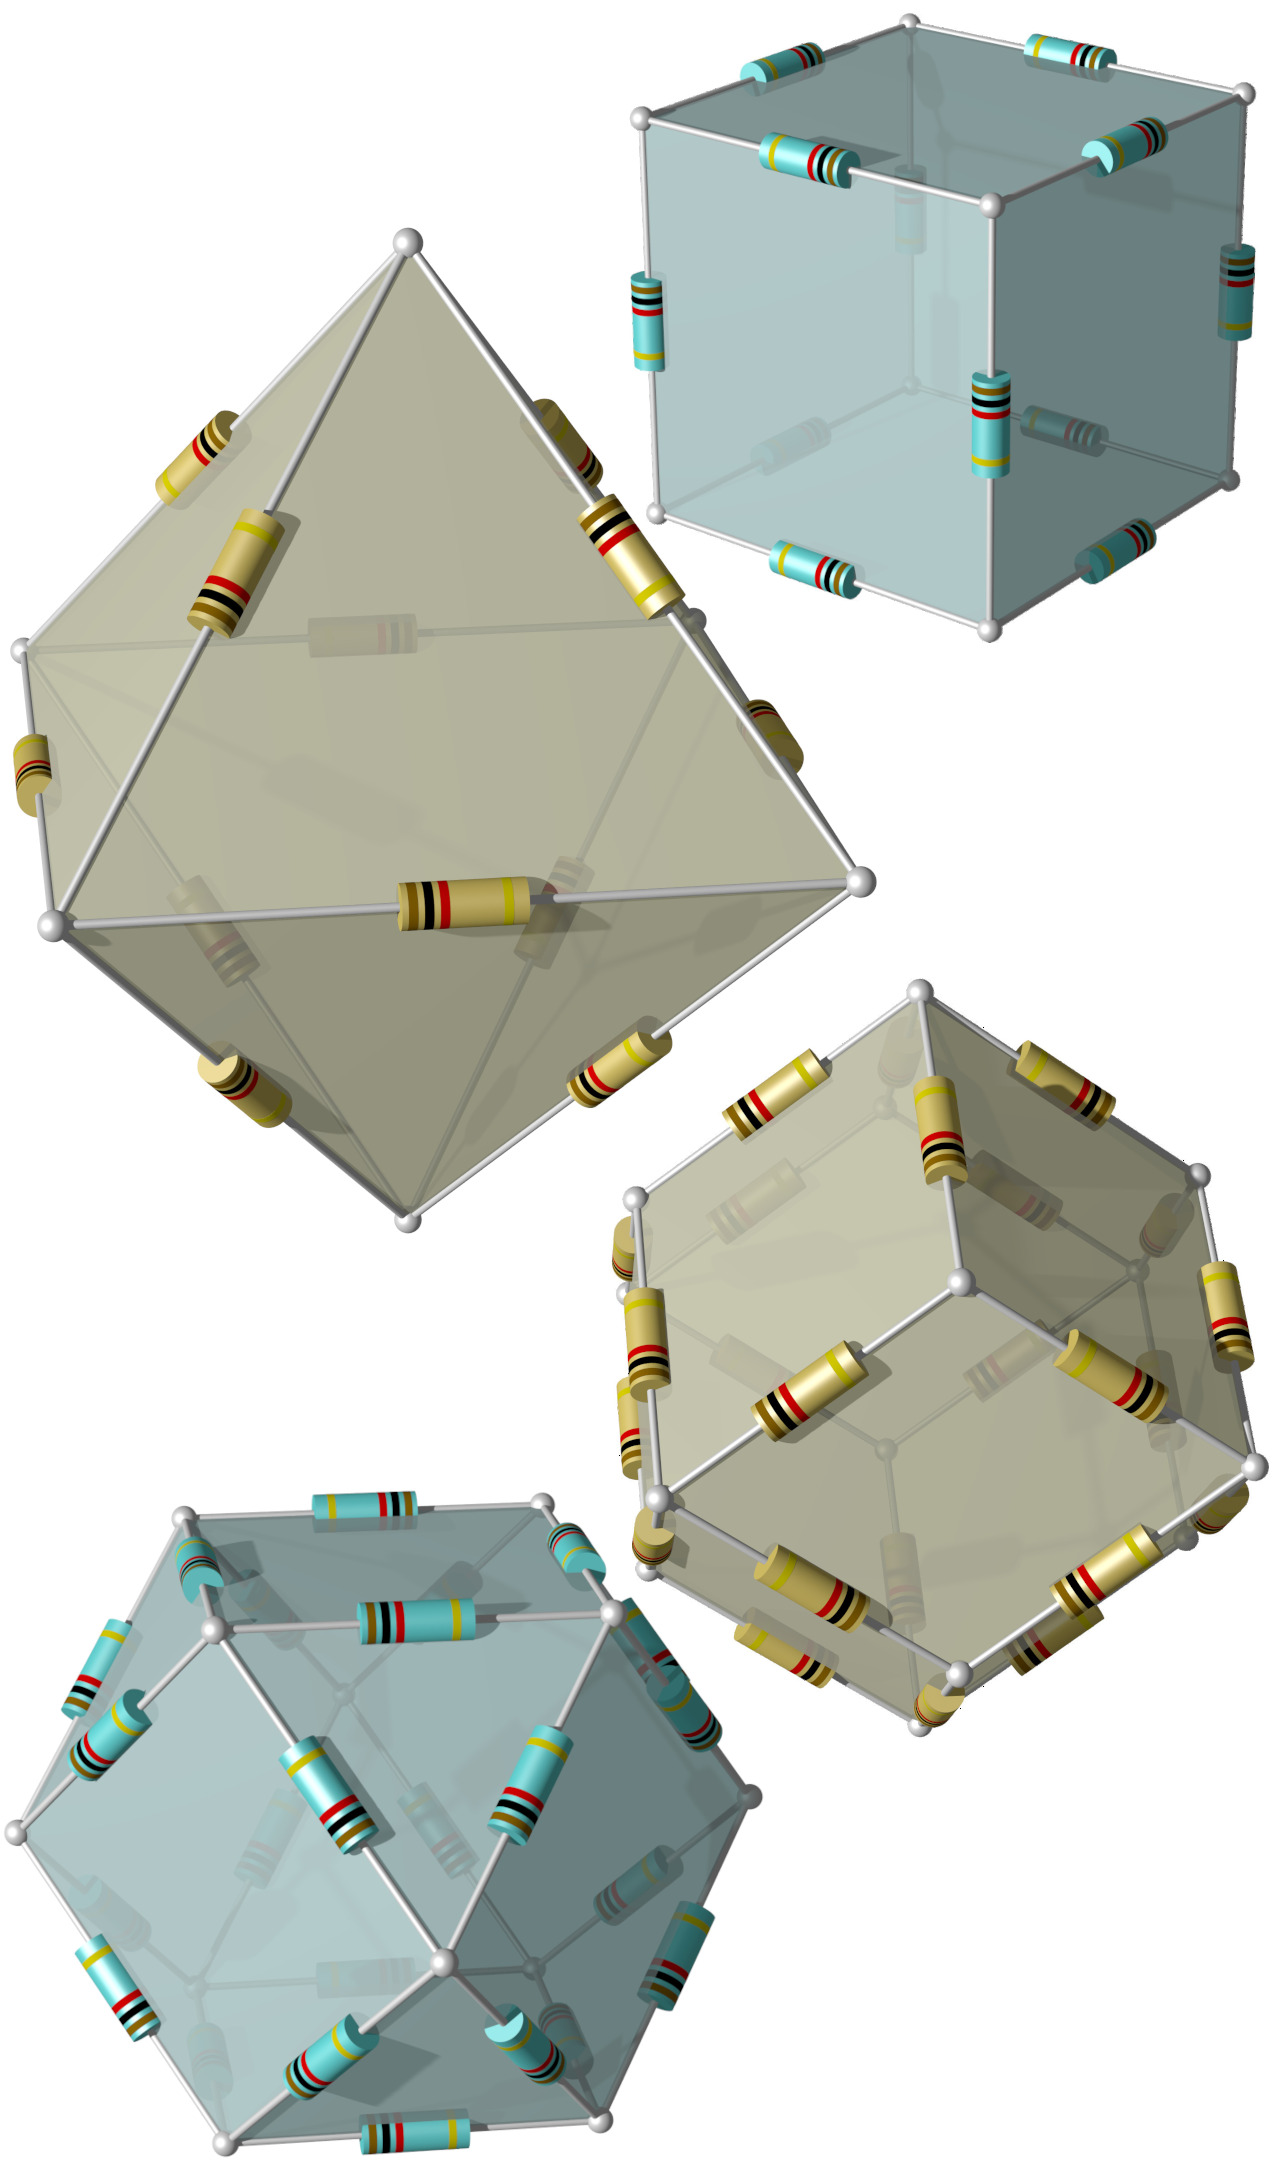
\includegraphics[width=0.8\textwidth]{../slides/6/punktgruppen/toi/O.jpg}
\end{center}
\end{block}}
\end{column}
\begin{column}{0.33\textwidth}
\uncover<3->{%
\begin{block}{$I = I_h \cap \operatorname{SO(3)}$}
\begin{center}
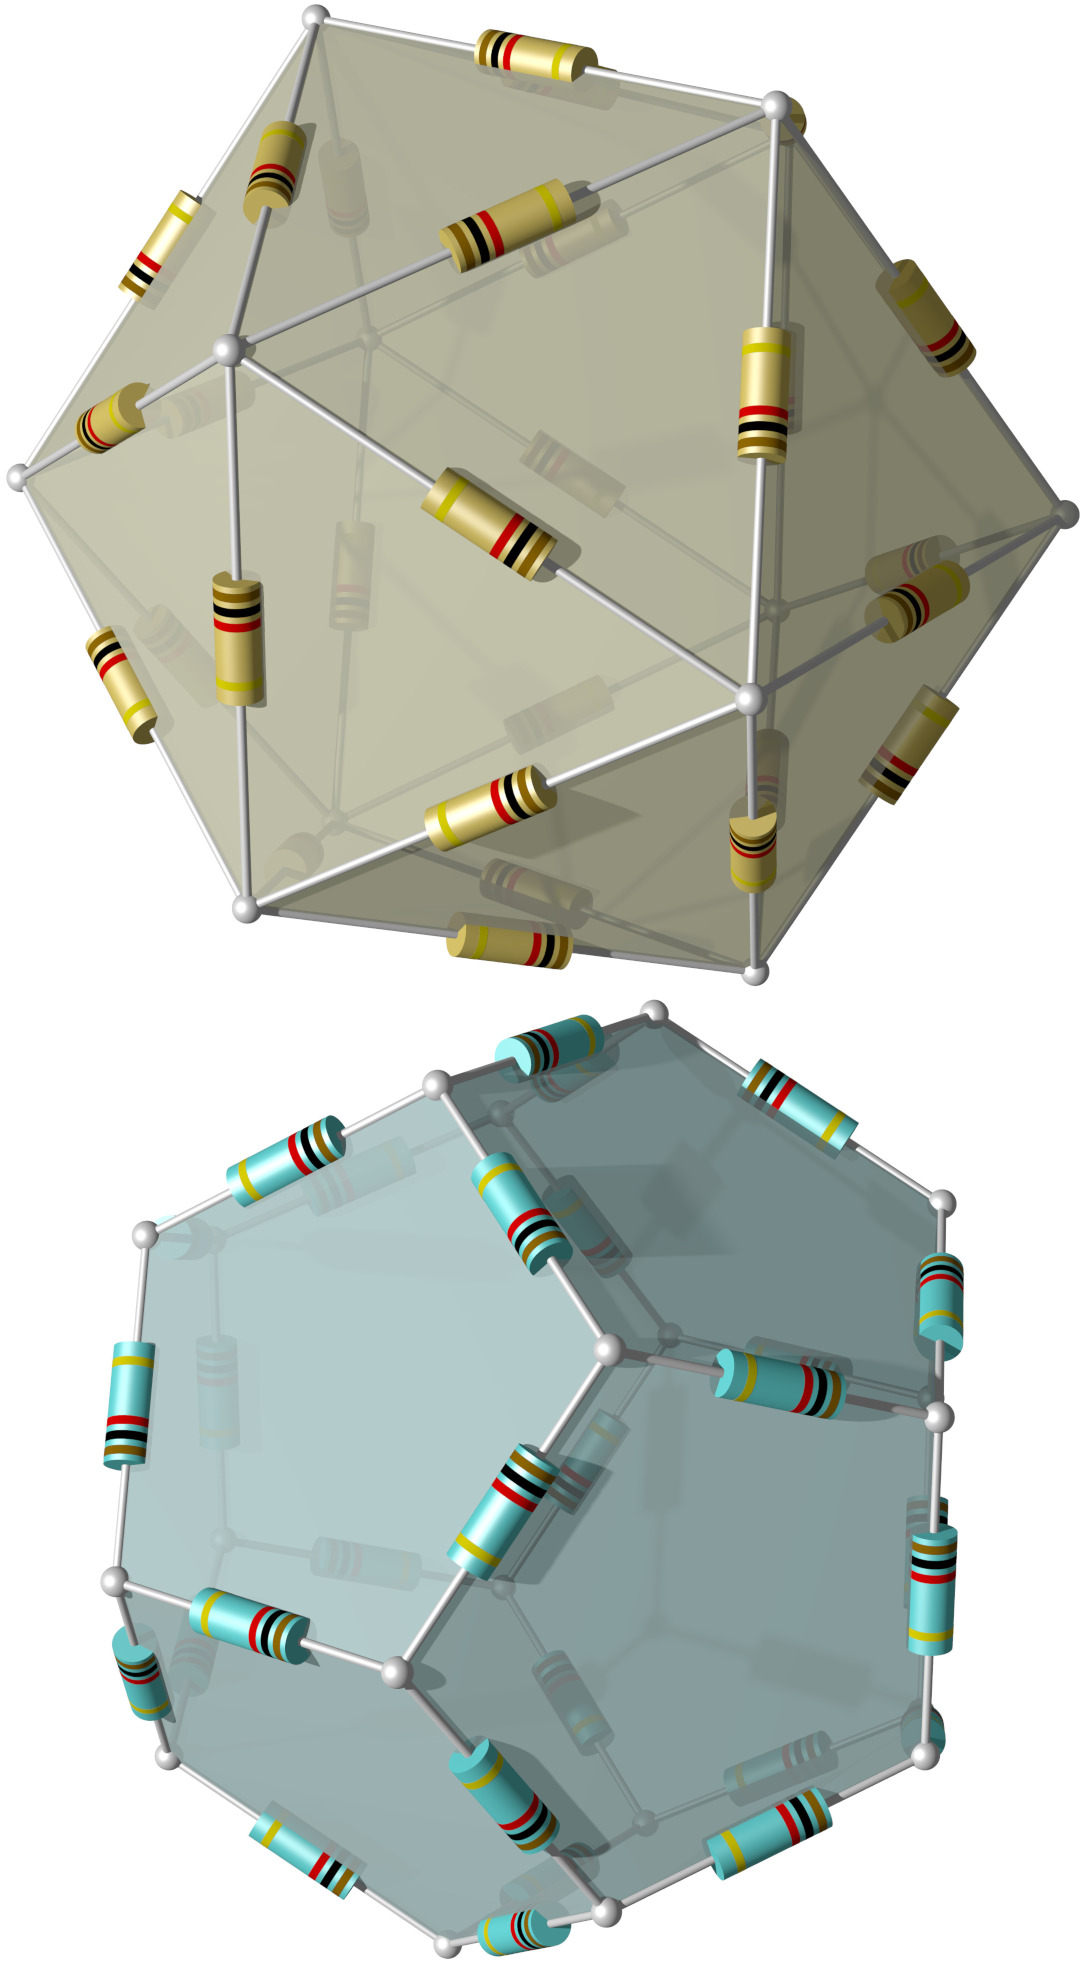
\includegraphics[width=0.8\textwidth]{../slides/6/punktgruppen/toi/I.jpg}
\end{center}
\end{block}}
\end{column}
\end{columns}
\end{frame}
\egroup
